\documentclass[11pt,a4paper]{article}
\usepackage{fontspec}
\usepackage{amsmath,amssymb}
\usepackage{tikz}
\usepackage{geometry}
\geometry{margin=18mm,top=20mm,bottom=20mm}
\usepackage{fancyhdr}
\usepackage[hidelinks]{hyperref}
\usepackage{xurl}
\definecolor{ink}{HTML}{182D3D}
\color{ink}
\pagestyle{fancy}\fancyhf{}\fancyhead[L]{\small ISEGORIA / INTEGRATION}\fancyhead[R]{\small 14 September 2026}\fancyfoot[R]{\thepage\ / 5}
\setlength{\parindent}{0pt}\setlength{\parskip}{7pt}
\newcommand{\topic}[1]{\vspace{6pt}{\large\bfseries #1}\par}
\newcommand{\pagetitle}[1]{{\LARGE\bfseries #1}\par\vspace{9pt}}
\setmainfont{Hiragino Mincho ProN}
\XeTeXlinebreaklocale "ja"
\XeTeXlinebreakskip=0pt plus 1pt
\begin{document}
\pagetitle{ルベーグ積分とリーマン積分}

リーマン積分は近い入力をまとめます。ルベーグ積分は同じ、あるいは近い出力をまとめ、それが現れる集合を測ります。同じ面積にたどり着く仕組みと、定義の違いが重要になる場面を探りましょう。

\begin{center}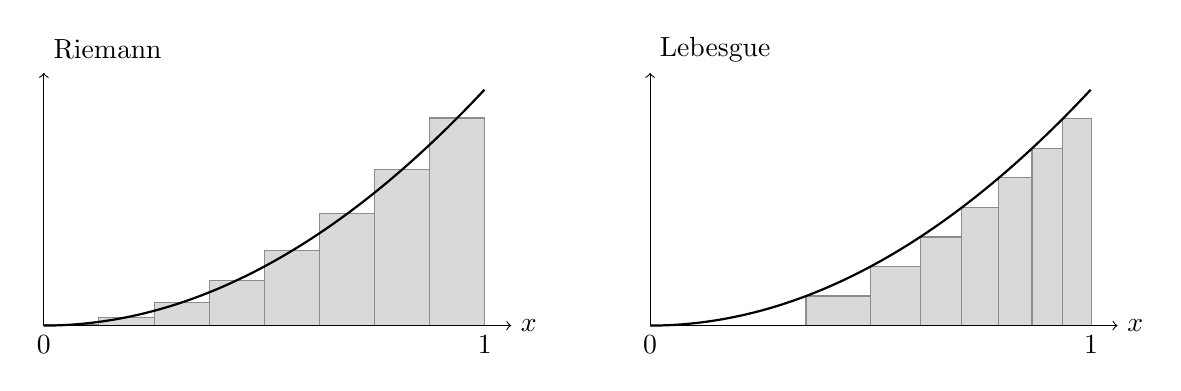
\begin{tikzpicture}[x=5.6cm,y=3.0cm]
\begin{scope}
\node[anchor=west] at (0,1.17) {Riemann};
\foreach \i in {0,...,7}{\pgfmathsetmacro{\a}{\i/8}\pgfmathsetmacro{\b}{(\i+1)/8}\pgfmathsetmacro{\h}{((\i+.5)/8)^2}\filldraw[fill=black!15,draw=black!45] (\a,0) rectangle (\b,\h);}
\draw[->] (0,0)--(1.06,0) node[right] {$x$};\draw[->](0,0)--(0,1.07);\draw[thick,domain=0:1,samples=70] plot (\x,{\x*\x});\node[below]at(0,0){$0$};\node[below]at(1,0){$1$};
\end{scope}
\begin{scope}[xshift=7.7cm]
\node[anchor=west] at (0,1.17) {Lebesgue};
\foreach \i in {0,...,7}{\pgfmathsetmacro{\a}{sqrt(\i/8)}\pgfmathsetmacro{\b}{sqrt((\i+1)/8)}\pgfmathsetmacro{\h}{\i/8}\filldraw[fill=black!15,draw=black!45] (\a,0) rectangle (\b,\h);}
\draw[->](0,0)--(1.06,0) node[right]{$x$};\draw[->](0,0)--(0,1.07);\draw[thick,domain=0:1,samples=70] plot (\x,{\x*\x});\node[below]at(0,0){$0$};\node[below]at(1,0){$1$};
\end{scope}\end{tikzpicture}\end{center}

\topic{図が表していること}

リーマン積分では \(a=x_0<\cdots<x_n=b\) と区間を分割し、各小区間から標本点 \(\xi_i\) を選んで和 S を作ります。有界関数がリーマン可積分であるとは、小区間の最大幅を 0 に近づけたとき、すべての標本点付きの和が同じ有限値に近づくことです。中点和の一つの列が収束するだけでは不十分です。

\[S(P,f)=\sum_{i=1}^n f(\xi_i)(x_i-x_{i-1}).\]

ルベーグ積分は、互いに素な可測集合 \(E_k\) 上の非負可測単関数 \(s=\sum_k a_k\mathbf{1}_{E_k}\) から始めます。その積分は \(\sum_k a_k\mu(E_k)\) です。集合は区間でなくてもかまいません。可測関数 \(f\ge0\) に対して、\(0\le s\le f\) を満たす単関数の積分の上限を \(\int f\,d\mu\) と定義します。値が無限大になることもあります。

\[\int f\,d\mu=\sup_{0\le s\le f,\ s\text{ simple}}\int s\,d\mu.\]

\newpage

\pagetitle{厳密な例と誤差評価}

この実験では \(0\le f\le1\) で、値の帯の幅は \(\frac1n\) です。最後の帯には値 1 も含めます。測度 1 の定義域上で \(0\le f-s\le 1/n\) なので、\(\int s\,d\mu\le\int f\,d\mu\le\int s\,d\mu+\frac1n\) となります。細分化は二等分を繰り返します。集合の長さは解析的に計算し、表示値は丸めています。

\topic{$f(x)=x^2$, $n=4$}

中点和は\[\frac{(1/8)^2+(3/8)^2+(5/8)^2+(7/8)^2}{4}=\frac{21}{64}=0.328125,\qquad \int_0^1x^2\,dx=\frac13.\]

値の帯の逆像とその長さは

\[E_k=\left[\sqrt{\frac{k}{n}},\sqrt{\frac{k+1}{n}}\right),\quad \mu(E_k)=\sqrt{\frac{k+1}{n}}-\sqrt{\frac{k}{n}}.\]

最終区間には右端も含めます。\[\int s_4\,d\mu=\sum_{k=0}^3\frac{k}{4}\left(\sqrt{\frac{k+1}{4}}-\sqrt{\frac{k}{4}}\right)\approx0.231717.\]

\topic{$f(x)=1-|2x-1|$}

値の帯の逆像は、端点を除けば次の２区間です。

\[\left[\frac a2,\frac b2\right]\cup\left[1-\frac b2,1-\frac a2\right],\qquad \mu(E)=b-a.\]

したがって\[\int s_n\,d\mu=\frac{n-1}{2n},\qquad \int_0^1f(x)\,dx=\frac12.\]

\topic{関連する見方：水平な層}

非負可測関数 f には、層別表示 \(\int f\,d\mu=\int_0^\infty\mu(\{x:f(x)>t\})\,dt\) が成り立ちます。これは「層の厚さ × 超水準集合の長さ」を足す表現です。互いに素な値の帯に下端の値を掛ける方法とは区別してください。ルベーグ積分は、単に x と y を交換する操作ではありません。

\newpage

\pagetitle{リーマン積分が存在しない例}

\([0,1]\) 上で、x が有理数なら \(D(x)=1\)、無理数なら \(D(x)=0\) と定めます。これは関数の定義であり、コンピューターで忠実に描ける曲線ではありません。

\[D(x)=\mathbf1_{\mathbb Q\cap[0,1]}(x)=\begin{cases}1&x\in\mathbb Q,\\0&x\notin\mathbb Q.\end{cases}\]

ダルブーの下和は常に 0、上和は常に 1 です。有理数を標本点にすれば和は 1、無理数なら 0 となり、どれほど細分しても一致しません。リーマン積分は存在しません。

\[L(P,D)=0\ne1=U(P,D),\qquad \int D\,d\mu=0.\]

\([0,1]\) の有理数は可算で、各一点のルベーグ測度は 0 です。可算加法性から \(\mu(\mathbb Q\cap[0,1])=0\)。したがって \(\int D\,d\mu=1\cdot0=0\) です。

\topic{測度 0 は「空」を意味しません}

有理数を \(q_1,q_2,\ldots\) と列挙します。任意の \(\varepsilon>0\) に対し、\(q_j\) を長さ \(\varepsilon/2^j\) の区間で覆います。すべての有理数を覆う区間の長さの合計は高々 \(\varepsilon\) です。\(\varepsilon\) をいくらでも小さくできるので測度は 0 です。稠密性と測度は、異なる性質を表します。

\topic{二つの積分が一致する条件}

コンパクト区間上の有界関数がリーマン可積分であることと、その不連続点の集合のルベーグ測度が 0 であることは同値です。リーマン可積分ならルベーグ可積分でもあり、積分値は一致します。至る所で連続であることは十分条件ですが、必要条件ではありません。

\topic{符号付き関数と広義積分}

実可測関数 f に対して \(f^+=\max(f,0)\)、\(f^-=\max(-f,0)\) とします。有限のルベーグ積分には \(\int|f|\,d\mu<\infty\) が必要で、積分は \(\int f^+\,d\mu-\int f^-\,d\mu\) です。一方だけが無限大なら拡張値を扱えますが、\(\infty-\infty\) は未定義です。条件収束する広義リーマン積分が、有限のルベーグ積分になるとは限りません。

\newpage

\pagetitle{大きな利点：極限を扱う}

\topic{優収束定理}

可測関数 \(f_n\) が f にほとんど至る所で収束し、単一の可積分関数 \(g\ge0\) に対して \(|f_n|\le g\) がほとんど至る所で成り立つなら、f は可積分で \(\int f_n\,d\mu\to\int f\,d\mu\) です。同じ g がすべての n に使える必要があります。

\topic{$f_n(x)=x^n$}

すべての項は可積分関数 1 以下です。極限はほとんど至る所で 0 となります。

\[f_n(x)\longrightarrow\mathbf1_{\{1\}}(x),\qquad\int_0^1x^n\,dx=\frac1{n+1}\longrightarrow0.\]

\topic{$f_n(x)=n\,\mathbf1_{(0,1/n)}(x)$}

各点で 0 に収束しますが、積分は 1 のままです。共通の可積分な優関数は存在しません。

\[\int_0^1 f_n(x)\,dx=n\cdot\frac1n=1\not\longrightarrow0=\int_0^1\lim_{n\to\infty}f_n(x)\,dx.\]

\topic{単調収束定理}

可測関数が \(0\le f_n\le f_{n+1}\) を満たし、f にほとんど至る所で収束するなら、\(\int f_n\,d\mu\) は \(\int f\,d\mu\) へ単調に増加します。\(+\infty\) も許されます。スパイクの列は単調増加ではなく、この仮定を満たしません。

\[0\le f_n\uparrow f\quad\Longrightarrow\quad\int f_n\,d\mu\uparrow\int f\,d\mu.\]

ルベーグ積分は数値求積を常に高速化する方法ではありません。重要なのは、可測集合と極限を統一的に扱えることです。

\newpage

\pagetitle{理解を確かめる}

\topic{1. 中点和の収束だけでリーマン可積分といえますか？}

いいえ。分割の最大幅が 0 に近づくとき、任意の分割と標本点で収束する必要があります。特定の標本点の選び方では、可積分性を妨げる挙動を見落とすことがあります。

\topic{2. 零集合上の値を変えてもリーマン可積分性は保たれますか？}

必ずしも保たれません。零関数の値をすべての有理数で 1 に変えると、ルベーグ積分は 0 のままですが、得られるディリクレ関数はリーマン可積分ではありません。

\topic{3. スパイクを共通に抑える可積分関数がないのはなぜ？}

もし存在すれば、優収束定理から積分は 0 に収束するはずです。しかし積分は常に 1 なので矛盾します。各スパイクは可積分です。不足しているのは、列全体に共通する上界の条件です。

\topic{参考文献と扱う範囲}

以下の大学講義ノートを参照した独自の解説と計算図です。この実験では \([0,1]\) 上の通常のルベーグ測度（長さ）を使います。抽象的な測度や非可測関数は扱いません。

\begin{itemize}\item MIT 18.125, Measure and Integration (2003), lectures 2--5. \url{https://ocw.mit.edu/courses/18-125-measure-and-integration-fall-2003/pages/lecture-notes/}\item Princeton MAT425, Measure Theory (2025). \url{https://web.math.princeton.edu/~js129/PDFs/teaching/MAT425_spring_2025/MAT425_Lecture_Notes.pdf}\end{itemize}

\url{https://theisegoria.github.io/ja/lebesgue-vs-riemann/}

英語原文。日本語版は AI の支援による翻訳です。

\end{document}

